\chapter{Lec 06 - Linear Regression}

\section{Linear Regression}
Linear regression is a simple approach to supervised learning. It assumes that the dependence of $Y$ on $X_1, X_2, . . . X_p$ is linear. Although it may seem overly simplistic, linear regression is extremely useful both conceptually and practically. Consider the following advertising data:
\begin{center}
    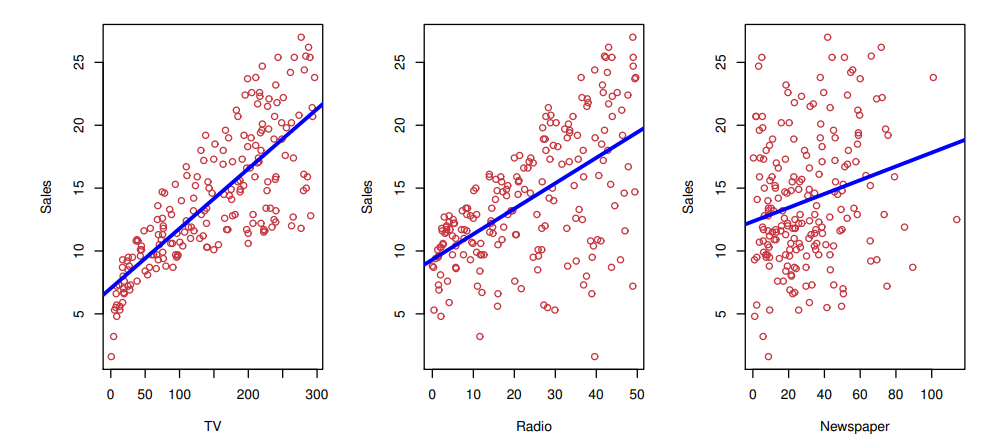
\includegraphics[scale=0.7]{images/advertising_lr.png}
\end{center}
Suppose that in our role as statistical consultants we are asked to suggest, on the basis of this data, a marketing plan for next year that will result in high product sales. What information would be useful in order to provide such a recommendation? Here are a few important questions that we might seek to address:
\begin{enumerate}
    \item Is there a relationship between advertising budget and sales?

    \item How strong is the relationship between advertising budget and sales?

    \item Which media contribute to sales?

    \item How accurately can we predict future sales?

    \item Is the relationship linear?

    \item Is there synergy among the advertising media?
\end{enumerate}
\textit{Simple linear regression} lives up to its name: it is a very straightforward approach for predicting a quantitative response $Y$ on the basis of a single predictor variable $X$. It assumes that there is approximately a linear relationship between $X$ and $Y$. Mathematically, we can write this linear relationship as:
\[Y \approx \beta_0 + \beta_1 X\]
For example, $X$ may represent TV advertising and $Y$ may represent sales. $\beta_0$ and $\beta_1$ are two unknown constants that represent
the \textit{intercept} and \textit{slope} terms in the linear model. Together, $\beta_0$ and $\beta_1$ are known as the model \textit{coefficients} or \textit{parameters}. Once we have used our training data to produce estimates $\hat{\beta}_0$ and $\hat{\beta}_1$ for the model coefficients, we can predict future sales on the basis of a particular value of TV advertising by computing
\[\hat{y} = \hat{\beta}_0 + \hat{\beta}_1 x\]
where $\hat{y}$ indicates a prediction of $Y$ on the basis of $X = x$.

\section{Estimating the Coefficients}
Let $\{(x_1, y_1), (x_2, y_2), ..., (x_n, y_n)\}$ be the $n$ observation pairs. Let $\hat{y}_i = \hat{\beta}_0 + \hat{\beta}_1 x_i$ be the prediction for $Y$ based on the $i$-th value of $X$. Then $e_i = y_i - \hat{y}_i$ represents the $i$-th residual, that is,  the difference between the $i$-th observed response value and the $i$-th response value that is predicted by our linear model. We define the residual sum of squares (RSS) as
\[\text{RSS} = e_1^2 + e_2^2 + ... + e_n^2\]
or equivalently as
\[\text{RSS} = (y_1 - \hat{\beta}_0 + \hat{\beta}_1 x_1)^2 + (y_2 - \hat{\beta}_0 + \hat{\beta}_1 x_2)^2 + ... + (y_n - \hat{\beta}_0 + \hat{\beta}_1 x_n)^2\]
The least squares approach chooses $\hat{\beta}_0$ and $\hat{\beta}_1$ to minimize the RSS. Using some calculus, one can show that the minimizers are
\[
\begin{split}
    \hat{\beta}_1 = & \frac{\sum_{i=1}^n (x_i - \overline{x}) (y_i - \overline{y})}{\sum_{i=1}^n (x_i - \overline{x})^2} \\
    \hat{\beta}_0 = & \overline{y} - \hat{\beta}_1 \overline{x}
\end{split}
\]
where $\overline{y} \equiv \frac{1}{n}\sum_{i=1}^n y_i$ and $\overline{x} \equiv \frac{1}{n}\sum_{i=1}^n x_i$ are the sample means.
\begin{center}
    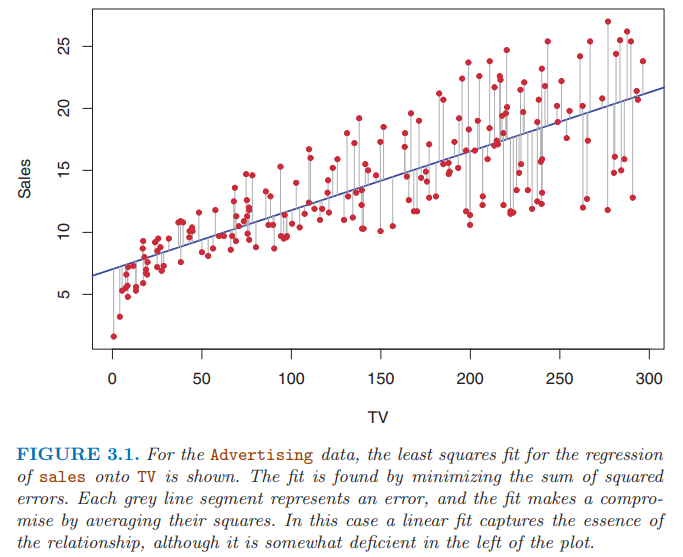
\includegraphics[scale=0.8]{images/linear_reg adv.png}
\end{center}

\section{Assessing the Accuracy of the Coefficient Estimates}
Recall that we assume that the true relationship between $X$ and $Y$ takes the form $Y = f(X) + \epsilon$ for some unknown function $f$, where $\epsilon$ is a mean-zero random error term. If $f$ is to be approximated by a linear function, then we can write this relationship as
\begin{equation}
    Y = \beta_0 + \beta_1X + \epsilon
    \label{pop_regr}
\end{equation}
Here $\beta_0$ is the intercept term, that is, the expected value of $Y$ when $X = 0$,
and $\beta_1$ is the slope, the average increase in $Y$ associated with a one-unit increase in $X$.\\\\
The model given by \ref{pop_regr} defines the \textit{population regression line}, which is the best linear approximation to the true relationship between $X$ and $Y$. The least squares regression coefficient estimates characterize the \textit{least squares line}.
\begin{center}
    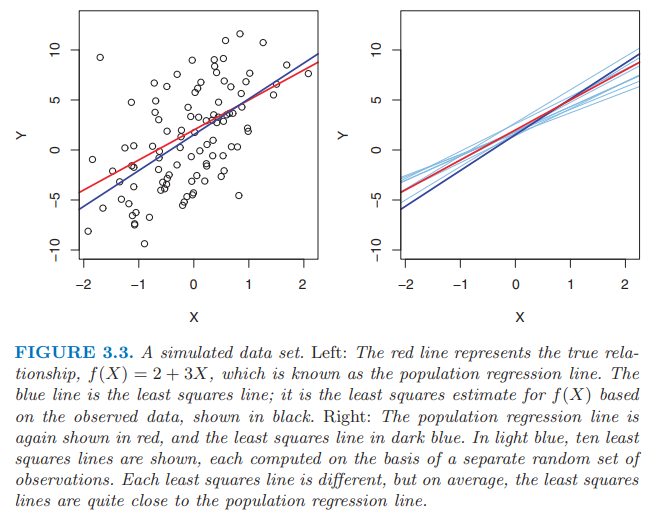
\includegraphics[scale=0.8]{images/pop_reg vs lsr.png}
\end{center}
At first glance, the difference between the population regression line and the least squares line may seem subtle and confusing. We only have one data set, and so what does it mean that two different lines describe the relationship between the predictor and the response? Fundamentally, the concept of these two lines is a natural extension of the standard statistical approach of using information from a sample to estimate characteristics of a large population.\\\\
For example, suppose that we are interested in knowing the population mean $\mu$ of some random variable $Y$.  Unfortunately, $\mu$ is unknown, but we do have access to $n$ observations from $Y$, which we can write as $y_1,...,y_n$, and which we can use to estimate $\mu$. A reasonable estimate is $\hat{\mu} = \overline{y}$, where $\overline{y} = \frac{1}{n}\sum_{i=1}^n y_i$ is the sample mean. The sample mean and the population mean are different, but in general the sample mean will provide a good estimate of the population mean. In the same way, the unknown coefficients $\beta_0$ and $\beta_1$ in linear regression define the population regression line. We seek to estimate these unknown coefficients using $\hat{\beta}_0$ and $\hat{\beta}_1$.\\\\
We continue the analogy with the estimation of the population mean
$\mu$ of a random variable $Y$. A natural question is as follows: how accurate is the sample mean $\hat{\mu}$ as an estimate of $\mu$?  the average of $\hat{\mu}$’s over many data sets will be very close to $\mu$, but that a single estimate $\hat{\mu}$ may be a substantial underestimate or overestimate of $\mu$. How far off will that single estimate of $\hat{\mu}$ be?  In general, we answer this question by computing the standard error of $\hat{\mu}$, written as $\text{SE}(\hat{\mu})$.
\[\text{Var}(\hat{\mu}) = \text{SE}(\hat{\mu})^2 = \frac{\sigma^2}{n}\]
Roughly speaking, the standard error tells us the average amount that this estimate $\hat{\mu}$ differs from the actual value of $\mu$. In a similar vein, we can wonder how close $\hat{\beta}_0$
and $\hat{\beta}_1$ are to the true values $\beta_0$ and $\beta_1$. To compute the standard errors
associated with $\hat{\beta}_0$ and $\hat{\beta}_1$, we use the following formulas:
\[\text{SE}(\hat{\beta}_0)^2 = \sigma^2 \left[ \frac{1}{n} + \frac{\overline{x}^2}{\sum_{i=1}^n (x_i - \overline{x})^2}\right], \quad \text{SE}(\hat{\beta}_1)^2 = \frac{\sigma^2}{\sum_{i=1}^n (x_i - \overline{x})^2}\]
where $\sigma^2 = \text{Var}(\epsilon)$\\\\
Standard errors can be used to compute confidence intervals. A 95\% confidence interval is defined as a range of values such that with 95\% probability, the range will contain the true unknown value of the parameter. For linear regression, the 95\% confidence interval for $\beta_1$
approximately takes the form
\[\hat{\beta}_1 \pm 2 \cdot \text{SE}(\hat{\beta}_1)\]
That is, there is approximately a 95\% chance that the interval
\[\left[\hat{\beta}_1 - 2 \cdot \text{SE}(\hat{\beta}_1), \,\, \hat{\beta}_1 + 2 \cdot \text{SE}(\hat{\beta}_1)\right]\]
will contain the true value of $\beta_1$. Similarly, a confidence interval for $\beta_0$ approximately takes the form
\[\hat{\beta}_0 \pm 2 \cdot \text{SE}(\hat{\beta}_0)\]
For the advertising data, the 95\% confidence interval for $\beta_1$ is $[0.042, 0.053]$.\\\\
Standard errors can also be used to perform hypothesis tests on the coefficients. The most common hypothesis test involves testing the \textit{null hypothesis} of
\[H_0 \,\, :\,\, \text{There is no relationship between $X$ and $Y$}\]
versus the \textit{alternative hypothesis}
\[H_A \,\, : \,\, \text{There is some relationship between $X$ and $Y$}\]
Mathematically, this corresponds to testing
\[H_0 \,\, : \,\, \beta_1 = 0\]
versus
\[H_A \,\, : \,\, \beta_1 \neq 0\]
since if $\beta_1 = 0$ then the model reduces to $Y = \beta_0 + \epsilon$, and $X$ is
not associated with $Y$. To test the null hypothesis, we need to determine whether $\hat{\beta}_1$, our estimate for $\beta_1$, is sufficiently far from zero that we can be confident that $\beta_1$ is non-zero. How far is far enough? This of course depends on the accuracy of $\hat{\beta}_1$, that is, it depends on $\text{SE}(\hat{\beta}_1)$. If $\text{SE}(\hat{\beta}_1)$ is small, then even relatively small values of $\hat{\beta}_1$ may provide strong evidence that $\beta_1 \neq 0$, and hence that there is a relationship between $X$ and $Y$. In contrast, if $\text{SE}(\hat{\beta}_1)$ is large, then $\hat{\beta}_1$ must be large in absolute value in order for us to reject the null hypothesis. In practice, we compute a $t$-statistic, given by
\begin{equation}
    t = \frac{\hat{\beta}_1 - 0}{\text{SE}(\hat{\beta}_1)}
    \label{t-stat}
\end{equation}
which measures the number of standard deviations that $\hat{\beta}_1$ is away from 0. If there really is no relationship between $X$ and $Y$ (i.e. assuming $\beta_1 = 0$), then we expect that \ref{t-stat} will have a $t$-distribution with $n - 2$ degrees of freedom.
\begin{center}
    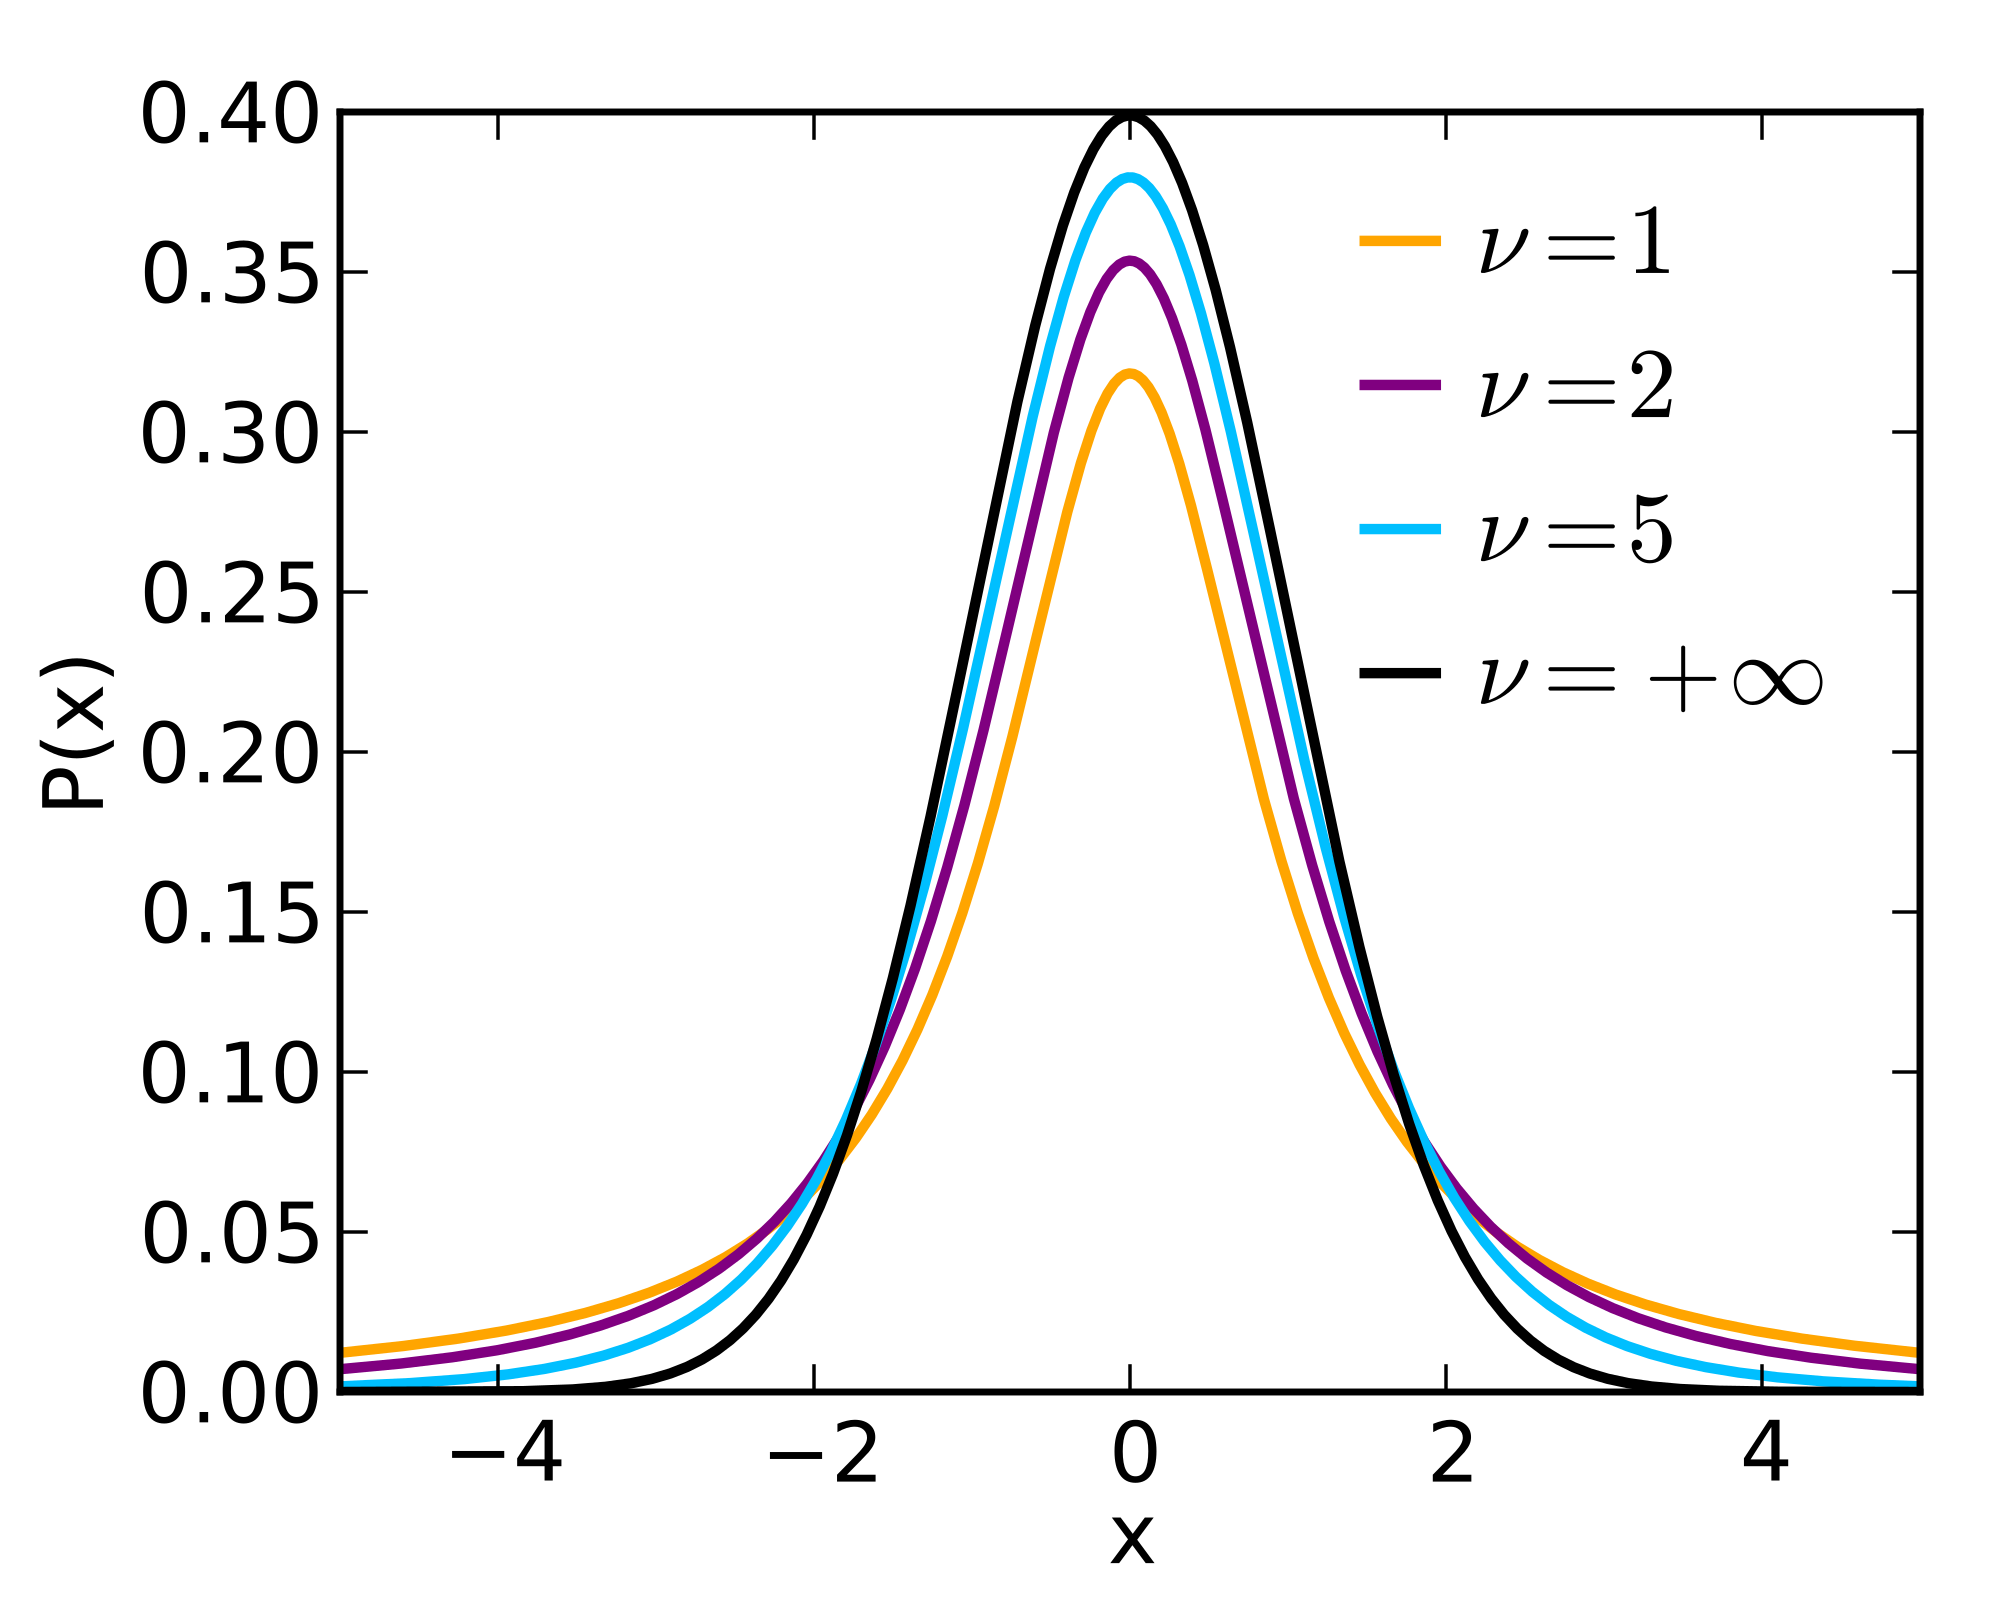
\includegraphics[scale=0.1]{images/t-distr.png}
\end{center}
The $t$-distribution has a bell shape and for values of $n$ greater than approximately 30 it is quite similar to the normal distribution. Consequently, it is a simple matter to compute the probability of observing any value equal to $|t|$ or larger, \textbf{assuming} $\beta_1 = 0$. We call this probability the $p$-value, which we can interpret as follows: \textit{which is the probability that the true $\beta_1$ is 0 if our estimate $\hat{\beta}_1$ is far from 0 according to $t$?} Note that if $\hat{\beta}_1$ is very close to 0 and/or $\text{SE}(\hat{\beta})_1$ is very high, then $t$ will be higher, and so the $p$-value. In contrast, if $\hat{\beta}_1$ is far from 0 and/or the standard error is very low, the $p$-value will be low.
\\\\
Hence, if we see a small $p$-value, then we can infer that there is an association between the predictor and the response. We reject the null hypothesis, that is, we declare a relationship to exist between $X$ and $Y$, if the $p$-value is small enough. Typical $p$-value cutoffs for rejecting the null hypothesis are 5 or 1\%.
\begin{center}
    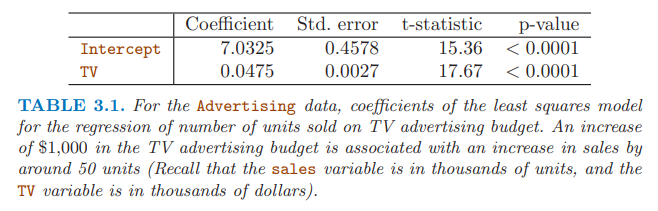
\includegraphics[scale=0.8]{images/p-value table.png}
\end{center}

